\documentclass{bioinfo}

\copyrightyear{2007}

\pubyear{2007}


\usepackage{amsfonts}
\usepackage{amssymb}
\usepackage{amsmath}

% to make citations:
% \citep{Bag01} = (Bag et al., 2001)
% \citealp{Bag01} = Bag et al., 2001


% Figures:
%\begin{figure}
%\centerline{\includegraphics{fig01.eps}}
%\caption{Caption, caption.}\label{fig:01}
%\end{figure}


% Table
%\begin{table}[t]
%\processtable{This is table caption\label{Tab:01}}
%{\begin{tabular}{llll}\toprule
%head1 & head2 & head3 & head4\\\midrule
%row1 & row1 & row1 & row1\\
%row2 & row2 & row2 & row2\\
%row3 & row3 & row3 & row3\\
%row4 & row4 & row4 & row4\\\botrule
%\end{tabular}}{This is a footnote}
%\end{table}


\def\RR{\mathbb{R}}
\newcommand {\OMIT}[1]{}
\newcommand {\todo}[1]{{\bf TODO: #1}}
\newcommand {\br}[1]{\left(#1\right)}
\newcommand {\nm}[1]{\Arrowvert\, #1 \,\Arrowvert}
\newcommand {\inpH}[2]{\left\langle #1 \right\rangle_{#2}}


\begin{document}

\firstpage{1}

\title[BiNoM Cytoscape plugin]{BiNoM: a Cytoscape plugin for manipulating and analyzing biological networks}
\author[Zinovyev and Viara]{Andrei Zinovyev\ $^{\rm a}$, Eric Viara\ $^{\rm a}$, Laurence Calzone\ $^{\rm a}$ and Emmanuel Barillot\ $^{\rm a}$}
\address{$^{\rm a}$Institut Curie, Service de Bioinformatique, 26 rue d'Ulm, F-75248 Paris Cedex 05, France}


\maketitle


\begin{abstract}

BiNoM (BIological NetwOrk Manager) is a new bioinformatics
software which significantly facilitates the usage and the
analysis of biological networks in standard systems biology
formats (SBML, SBGN, BioPAX). BiNoM implements a full-featured
BioPAX editor and a method of ``interfaces'' for accessing BioPAX
content. BiNoM is able to work with huge BioPAX files such as
whole pathway databases. In addition, BiNoM allows the analysis of
networks created with CellDesigner software and their conversion
into BioPAX format. BiNoM comes as a library and as a Cytoscape
plugin which adds a rich set of operations to Cytoscape such as
path and cycle analysis, clustering sub-networks, decomposition of
network into modules, clipboard operations and others.

\section{Availability:} Last version of BiNoM distributed under the LGPL licence
together with documentation, source code and API are available at
\href{http://bioinfo.curie.fr/projects/binom}
 {http://bioinfo.curie.fr/projects/binom}


\section{Contact:} \href{andrei.zinovyev@curie.fr}{andrei.zinovyev@curie.fr, binom@curie.fr}
\end{abstract}


\section{Introduction}

Importance of biological network knowledge standardization and
representation is widely accepted in the systems biology community
\cite{Klipp2007}. Several standards with different specialties
(e.g. SBML and BioPAX) have been proposed and are actively
promoted in many softwares \cite{Stromback2005}, such as
CellDesigner in which the Systems Biology Graphical Notation
standard (SBGN, http://sbgn.org) was proposed and implemented
\cite{Celldesigner2005}.

The Cytoscape environment \cite{Cytoscape2003} is an open-source
project aimed at creating universal and flexible biological
network visualization tool. It has attracted a lot of attention
and collected a large and active community around it due to the
possibility of extending its base functionality with user-made
plugins. A number of plugins are already developed and used in
practice (see the list at http://cytoscape.org). In the recent
versions of Cytoscape there is an option to import BioPAX and SBML
files, however, these capabilities remain limited to a simple
visualization of the file content.

\begin{figure*}
\centerline{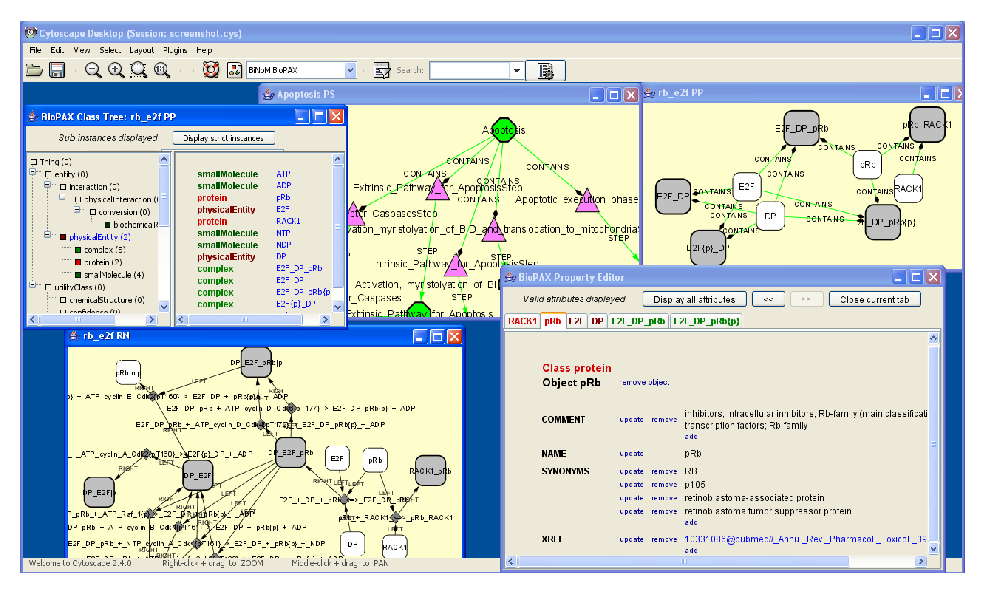
\includegraphics[width=18cm,
height=8cm]{screenshot.eps}} \caption{\label{screenshot} BiNoM
screenshot. Three standard BioPAX interfaces (RN, PS, PP), BioPAX
property editor and BioPAX class tree dialog are shown. RN and PP
visualize small BioPAX file describing RB-E2F interaction, PS
shows pathway structure for Apoptosis pathway from Reactome DB. }
\end{figure*}


BiNoM (BIological NetwOrk Manager) plugin was developed to
facilitate manipulating files in BioPAX and SBML formats
(including CellDesigner SBML extension). BiNoM allows to read,
edit, extract parts, merge and save systems biology files.
Together with this function, a large set of structure analysis
tools is proposed. In addition, BiNoM supports conversion of
CellDesigner to BioPAX and BioPAX to SBML formats. BiNoM was used
in several projects on analyzing complex biological networks (for
example, see \cite{RbPathway}).

\section{Methods and Implementation}

The first guiding principle of BiNoM is to provide control in
Cytoscape over the content of a systems biology file without
complete conversion of the file into the Cytoscape internal
format. Second, BiNoM aims at dissecting and reducing the
complexity of the visual network presentation with help of a
number of graph structural analysis methods, some of them taking
into account the biological semantics connected to the graph
elements.

To access the content of a file, the BiNoM engine first maps it
onto a labeled directed graph, called {\it index}. Index
represents the totality of objects and their relations, but with a
minimum amount of information necessary for their visual
representation. The whole index is a highly connected graph which
is usually not visualized explicitly. The user interacts with
subgraphs extracted from the global index, called {\it network
interfaces}. For example, during BioPAX import operation, BiNoM
proposes to generate three standard interfaces: Reaction Network
(RN), Pathway Structure (PS) and Protein-Protein interaction (PP).
These subgraphs represent three different aspects of information
contained in BioPAX file (see Fig.~\ref{screenshot}). For full
description of a BiNoM data model, go to the BiNoM web-site.

%The Reaction Network interface is a bipartite graph composed of
%two types of nodes: reactions (shown by diamonds in
%Fig.~\ref{screenshot}) and chemical species. They are connected by
%edges of different types (LEFT for reactants, RIGHT for reaction
%products, CATALYSIS and MODULATION for modifier chemical species).
%The Pathway Structure interface represents the pathway structure
%contained in BioPAX. Here, nodes can either represent ``pathway'',
%``pathway step'' or ``interaction''. The Protein-Protein
%interaction interface visualizes the formation of proteins or
%protein complexes and other protein-protein interactions described
%in the BioPAX file.

Starting from these subgraphs and using operations proposed by
BiNoM such as copy-paste, graph merging and extracting graph
parts, the user can construct his or her own arbitrary interface.
Any node or edge in the interface can be assigned one or several
URI attributes which BiNoM uses to access and modify the file
content. To do so, the interface should be first {\it associated}
to the file through BiNoM menu. After that, the user can save the
whole object hierarchy or export to a file only a part of the
content represented in the interface. When doing this, it is
possible to merge the new information with already existing files.
The BioPAX Reaction Network interface can be exported to SBML
format and serve as a first draft for the creation of a pathway
computational model. Any interface or the whole index can be
stored as XGMML (standard labeled graph description format
supported by Cytoscape) file and used later.

%\begin{figure}
%\centerline{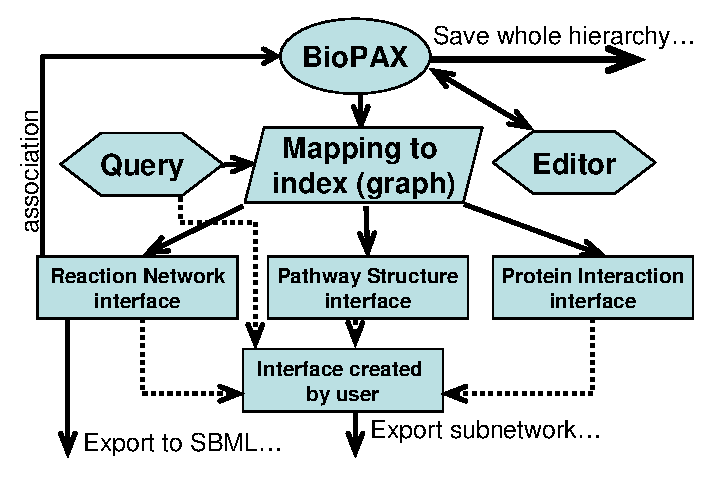
\includegraphics[width=5cm,
%height=3cm]{BioPAXdiagram.eps}} \caption{\label{BioPAXdiagram}
%Schema of working with BioPAX in BiNoM. Rectangles represent
%Cytoscape networks (interfaces) used to access BioPAX. }
%\end{figure}


If the BioPAX file is huge such as a whole pathway database (e.g.
Reactome \cite{Reactome2005}), the user can use the BiNoM querying
mechanism to extract part of the database and export it into a
separate self-containing BioPAX file for further analysis. This
mechanism enables using Cytoscape viewer and a big BioPAX file as
a pathway database with a flexible interface.

%The querying mechanism converts Cytoscape into a flexible local
%interface to a local pathway database stored as a big BioPAX file.
%In future developments, alternative ways of interacting with
%pathway databases will be provided.

Simplification and analysis of the network representation are
achieved by use of the build-in library of graph analysis tools,
including analysis of connected and strongly connected components,
path analysis (finding shortest, suboptimal, all paths), modular
decomposition of the network using node semantics, cycle analysis,
subnetwork clustering and clipboard operations.

The logic implementation in the BiNoM code is completely decoupled
from the Cytoscape interface. That way, BiNoM can be used as an
independent biological graph analysis library. Using run-time
object inspection in Java allows the reuse of BiNoM code with
practically any ontology schema, even completely different from
BioPAX (for example, Systems Biology Ontology). BiNoM was tested
with 2.3, 2.4 and 2.5 versions of Cytoscape and with 3.* versions
of CellDesigner.

\section*{Acknowledgments}

This project was partly funded by the EC contract ESBIC-D
(LSHG-CT-2005-518192), the PIC Bioinformatique et Biostatistiques
from Institut Curie, and the Research Networks Program in
Bioinformatics from the High Council for Scientific and
Technological Cooperation between France and Isra�l.

\bibliographystyle{plainnat}
%\bibliography{../refs/kernelchip}

\begin{thebibliography}{99}

%\bibitem{Cytoscape2003}Shannon, P., Markiel, A., Ozier, O., Baliga, N. S., Wang, J. T.,
%Ramage, D., Amin, N., Schwikowski, B., and Ideker, T. (2003).
%Cytoscape: a software environment for integrated models of
%biomolecular interaction networks. {\it Genome Res} {\bf 13},
%2498-2504.

\bibitem{Klipp2007}Klipp E. et al. (2007). Systems biology standards--the community speaks. {\it
Nat Biotechnol} {\bf 25}, 390-391.

\bibitem{Stromback2005}Stromback L. and Lambrix P. (2005). Representations of
molecular pathways: an evaluation of SBML, PSI MI and BioPAX. {\it
Bioinformatics} {\bf 21}, 4401-4407.

\bibitem{Celldesigner2005}Kitano H. et al. (2005).
Using process diagrams for the graphical representation of
biological networks. {\it Nat Biotechnol} {\bf 23}, 961-966.

\bibitem{Cytoscape2003}Shannon P. et al. (2003).
Cytoscape: a software environment for integrated models of
biomolecular interaction networks. {\it Genome Res} {\bf 13},
2498-2504.

\bibitem{RbPathway} Calzone L. et al. (2007) A Comprehensive Modular Map of Molecular
Interactions in RB/E2F Pathway. {\it Manuscript submitted}. See
\href{http://bioinfo.curie.fr/projects/rbpathway}
 {http://bioinfo.curie.fr/projects/rbpathway}

\bibitem{Reactome2005}Joshi-Tope G. et al. (2005). Reactome: a knowledgebase of
biological pathways. Nucleic Acids Res 33, D428-432.


\end{thebibliography}

%\bibliography{bibl}

\end{document}
